%========================================================================
%
%========================================================================

\section{The random generators}
\label{section:random-generator}

  In a simulator, the generation of random numbers is an important part. 
In {\sc ndes}, we take this very serious. The random number generator 
management is a nameless horror! I admit I had problems understanding it too. 
The good knews is that the result is really \ldots{} random.

%------------------------------------------------------------------------
%
%------------------------------------------------------------------------
\subsection{The characteristics of a random generator}

 A random generator is characterised by three important components:

\begin{description}
   \item[The type of generated data] can be real, integer,
     discrete, \ldots
   \item[The law] can be uniform, exponential, \ldots
   \item[The source] permits to determine the quality of the randomness, and 
by example to render it deterministic (to obtain the same sequence with other 
simulation).
\end{description}

  Be careful, these three components eventualy use some parameters.
  
    The general principle for generating a variable is described below.

\begin{itemize}
   \item A random number is provided by the source. It will be a
      integer between two extreme values​​, for example, depending on
      the nature of the source.
   \item A transformation is applied to meet the probability density 
      of the law.
   \item A second transformation is applied to obtain a
      value of the desired type.
\end{itemize}

   Shortly, everything is done to make the generation random \ldots


%------------------------------------------------------------------------
%
%------------------------------------------------------------------------
\subsection{Using the generators}

  The general schema for using the generator is simple: we create a generator,
we initialise with the desired values, we associate with it a probability 
distribution, eventualy we can change the source of randomness on which it is based,
then we can extract the random values and at the end we destroy the generator.

   Observe in detail relevant functions of this exciting program.

%------------------------------------------------------------------------
%
%------------------------------------------------------------------------
\subsection{The creation and the destruction}
   
   There is at least a function of creation for each type of
managed data (it fails more than that!). But sometimes, there are also
functions to specify the distribution to use at the same time. 
See this type per type.

%.......................................................................
%
%.......................................................................
\subsubsection{The unsigned integers}

   The function for creating the base is 

\index{randomGenerator\_createUInt}
\begin{verbatim}
struct randomGenerator_t * randomGenerator_createUInt();
\end{verbatim}

%.......................................................................
%
%.......................................................................
\subsubsection{The unsigned integers between {\tt min} and {\tt max}}

   It is fun to play dice. This can be created with

\begin{verbatim}
struct randomGenerator_t * randomGenerator_createUIntRange(unsigned int min,
						      unsigned int max);
\end{verbatim}

%.......................................................................
%
%.......................................................................
\subsubsection{A list of unsigned integers}

   Practice to randomize packet sizes!

\index{randomGenerator\_createUIntDiscrete}
\begin{verbatim}
struct randomGenerator_t * randomGenerator_createUIntDiscrete(int nbValues,
							      unsigned int * values);
\end{verbatim}

   The first parameter gives the number of values, and the second is 
a table which contains (at least) these values. Its contents will be
copied, so if you want to destroy / modify then, you're free to do it!
   As there is little doubt that in such situations we will
want to assign a probability to each value, you can use the
following version:

\index{randomGenerator\_createUIntDiscreteProba}
\begin{verbatim}
struct randomGenerator_t * randomGenerator_createUIntDiscreteProba(
				int nbValues,
				unsigned int * values,
				double * proba);
\end{verbatim}

%.......................................................................
%
%.......................................................................
\subsubsection{The real numbers in double precision}

   We create a generator with the following function

\index{randomGenerator\_createDouble}
\begin{verbatim}
struct randomGenerator_t * randomGenerator_createDouble();
\end{verbatim}

   We may also create one generator based on an exponential distribution
parameter {\tt lambda} :

\index{randomGenerator\_createDoubleExp}
\begin{verbatim}
struct randomGenerator_t * randomGenerator_createDoubleExp(double lambda);
\end{verbatim}

%.......................................................................
%
%.......................................................................
\subsubsection{The real numbers in double precision between {\tt min} and {\tt max}}

\begin{verbatim}
\end{verbatim}

%.......................................................................
%
%.......................................................................
\subsubsection{A list of real numbers in double precision}

   For generating random numbers from a list with provided
parameters:

\index{randomGenerator\_createDoubleDiscrete}
\begin{verbatim}
struct randomGenerator_t * randomGenerator_createDoubleDiscrete(
                                     int nbValues,
                                     double * values);
\end{verbatim}

   or, providing the probabilities directly:

\index{randomGenerator\_createDoubleDiscreteProba}
\begin{verbatim}
struct randomGenerator_t * randomGenerator_createDoubleDiscreteProba(
                                     int nbValues,
                                     double * values,
                                     double * proba);
\end{verbatim}

   The parameters are similar to the release based on unsigned short 
int, according on what we see above.

%.......................................................................
%
%.......................................................................
\subsubsection{The destruction}

   We destroy the generator with the function

\index{randomGenerator\_delete}
\begin{verbatim}
void randomGenerator_delete(struct randomGenerator_t * rg);
\end{verbatim}

%------------------------------------------------------------------------
%
%------------------------------------------------------------------------
\subsection{Choosing the distribution}

   Before it can be used, a random generator need to be characterised
by a law that governs it. There are specific functions for this
purpose. These functions look like this

\begin{verbatim}
void randomGenerator_setDistribution<dist>(struct randomGenerator_t * rg,
                                           <parameters>);
\end{verbatim}

   Where \lstinline!dist! is one of the available distributions (see
below) and \lstinline!parameters! is the list (possibly empty) of
parameters.

   The list of available distributions is given in section
\ref{subsection:distributions}. A distribution can also be define
from its quantile function.


   Some function of creation call either of these functions, but not all! 
So be careful to ensure that a distribution is associated with a generator 
before using it.

%........................................................................
%
%........................................................................
\subsubsection{Defining the distribution from quantile function}

   A distribution can be defined by its quantile function (the inverse
distributon function) when available. For this purpose, some functions
are provided :

\index{randomGenerator\_setQuantile1Param}
\index{randomGenerator\_setQuantile2Param}
\begin{verbatim}
void randomGenerator_setQuantile1Param(struct randomGenerator_t * rg,
				       double (*q)(double x, double p),
				       double p);
void randomGenerator_setQuantile2Param(struct randomGenerator_t * rg,
				       double (*q)(double x, double p1, double p2),
				       double p1, double p2);
\end{verbatim}

   Each of these functions sets the random generator's distribution
based on the quantile function given as parameter
\lstinline!q!. Parameters \lstinline!p! or \lstinline !p1! and
\lstinline!p2! are used for the evaluation of \lstinline!q!.

   For example, the function \lstinline!randomGenerator\_paretoDistQ!
is defined in \lstinline!random-generator.c! as 

\index{randomGenerator\_paretoDistQ}
\begin{verbatim}
double randomGenerator_paretoDistQ(double x, double alpha, double xmin)
{
   return  xmin/(pow(x, 1.0/alpha));
}
\end{verbatim}

   The Pareto distribution described in \ref{subsubsection:paretodist}
is then defined in \lstinline!random-generator.h! as 

\index{randomGenerator\_setDistributionPareto}
\begin{verbatim}
#define randomGenerator_setDistributionPareto(rg, alpha, xmin) \
   randomGenerator_setQuantile2Param(rg, randomGenerator_paretoDistQ, alpha, xmin)
\end{verbatim}

%------------------------------------------------------------------------
%
%------------------------------------------------------------------------
\subsection{Choosing the source}

%------------------------------------------------------------------------
%
%------------------------------------------------------------------------
\subsection{Generating a value}

\index{randomGenerator\_getNextUInt}
\index{randomGenerator\_getNextDouble}

   A new value is obtained at each call of the following functions 
(chosen according to the expected type)

\begin{verbatim}
unsigned int randomGenerator_getNextUInt(struct randomGenerator_t * rg);
double randomGenerator_getNextDouble(struct randomGenerator_t * rg);
\end{verbatim}

%------------------------------------------------------------------------
%
%------------------------------------------------------------------------
\subsection{Available distributions}
\label{subsection:distributions}

%.......................................................................
%
%.......................................................................
\subsubsection{Explicit law}
   
   I do not know how to call that! The idea is that it explicitly provides 
all the probabilities. It is specified by the following function:
   
\index{randomGenerator\_setDistributionDiscrete}
\begin{verbatim}
void randomGenerator_setDistributionDiscrete(struct randomGenerator_t * rg,
					     int nb,
                                             double * proba);
\end{verbatim}
   
   Attention, it obviously only applies to discrete data!

   The probabilities are copied by the functions so the pointer
{\tt proba} can be released.

%.......................................................................
%
%.......................................................................
\subsubsection{Uniform law}

   We specify a uniform law through the following function

\index{randomGenerator\_setDistributionUniform}
\begin{verbatim}
void randomGenerator_setDistributionUniform(struct randomGenerator_t * rg);
\end{verbatim}
   
   Be careful, the type of data can be a "continuous" bounded interval
or a discrete set, but if it is an unbounded interval, the result is
\ldots {} random.

   Figure \ref{figure:distuni} shows an example of a uniform real
distribution in $[0, 1]$.

\begin{figure}[h]
\begin{center}
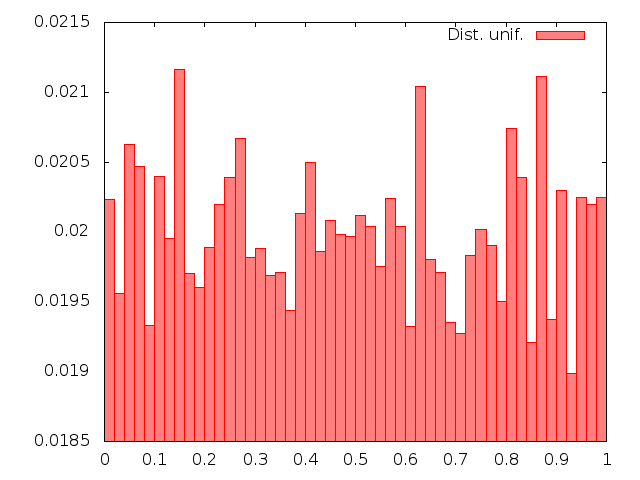
\includegraphics[width=0.5\textwidth]{DistributionUnif.png}
\caption{Uniform distribution example \label{figure:distuni}}
\end{center}
\end{figure}


%........................................................................
%
%........................................................................
\subsubsection{Pareto distribution}
\label{subsubsection:paretodist}

   A Pareto distribution with parameters  $\alpha$ et $x_{min}$  is
set to a random generator with the help of the following function

\index{randomGenerator\_setDistributionPareto}
\begin{verbatim}
void randomGenerator_setDistributionPareto(struct randomGenerator_t * rg,
                                           double alpha, double xmin);
\end{verbatim}

%........................................................................
%
%........................................................................
\subsubsection{Weibull distribution}
\label{weibull_dist}
\index{randomGenerator\_setDistributionWeibull}
\index{randomGenerator\_WeibullInit}
\index{randomGenerator\_WeibullGetNext}

   Weibull distribution is characterized by two parameters, $\alpha$
and $\beta$. To generate a random number based on Weibull
distribution, we need a random value, which we get from
rg->aleaGetNext. Then, we apply the inverse CDF of Weibull
distribution: 

  $$Weibull\_CDF^{-1}(x,\alpha,\beta)=\beta*(-\ln(1-x))^{1/\alpha}$$

\begin{verbatim}
void randomGenerator_setDistributionWeibull(struct randomGenerator_t * rg, double alpha, double beta)
{
   rg->distribution = rGDistWeibull;
   randomGenerator_WeibullInit(rg, alpha, beta);
}
\end{verbatim}


\begin{verbatim}
void randomGenerator_WeibullInit(struct randomGenerator_t * rg, double alpha, double beta)
{
      assert(rg->distribution == rGDistWeibull);   
      rg->distParam.min = 0.0;
      rg->distParam.max = DBL_MAX;
  
      rg->distParam.d.alpha = alpha;
      rg->distParam.d.beta  = beta; 
      rg->distGetNext = randomGenerator_WeibullGetNext;
}
\end{verbatim}

\begin{verbatim}
double randomGenerator_WeibullGetNext(struct randomGenerator_t * rg)
{
      double alea, result;
      alea = rg->aleaGetNext(rg);

        result = rg->distParam.d.beta *  pow(-log(1-alea), 
                                       1/rg->distParam.d.alpha);
     return result;
}
\end{verbatim}

%........................................................................
%
%........................................................................
\subsubsection{Lognormal distribution}
\label{lognormal_dist}
\index{randomGenerator\_setDistributionLognormal}
\index{randomGenerator\_LognormalInit}
\index{randomGenerator\_LognormalGetNext}

Lognormal distribution is characterized by two parameters, $\alpha$ and $\beta$.
To generate a random number based on Lognormal distribution, we need a random value, which we get from rg->aleaGetNext. Then, we apply the inverse CDF of Lognormal distribution:

   $$ Lognormal\_CDF^{-1}(x,\alpha,\beta) = e^{\alpha + \beta * sqrt{2} * errorfunction(2*x-1)^{-1}} $$

\begin{verbatim}
void randomGenerator_setDistributionLognormal(struct randomGenerator_t * rg, double alpha, double beta)
{
   rg->distribution = rGDistLognormal;
   randomGenerator_LognormalInit(rg, alpha, beta);
} 
\end{verbatim}

\begin{verbatim}
void randomGenerator_LognormalInit(struct randomGenerator_t *rg, double alpha, double beta)
{
      assert(rg->distribution == rGDistLognormal);   
      rg->distParam.min = 0.0;
      rg->distParam.max = DBL_MAX;
  
   rg->distParam.d.alpha = alpha;
   rg->distParam.d.beta  = beta; 
   rg->distGetNext = randomGenerator_LognormalGetNext;

}
\end{verbatim}

\begin{verbatim}
double randomGenerator_LognormalGetNext(struct randomGenerator_t *rg)
{  
      double alea;
      double result ;
   
   alea = rg->aleaGetNext(rg);

   result = exp (   rg->distParam.d.alpha + 
                    rg->distParam.d.beta * sqrt(2) * pow(erf(2*alea - 1), -1) 
                );

   return result;

}  
\end{verbatim}

%........................................................................
%
%........................................................................
\subsubsection{Gamma distribution}
\label{gamma_dist}
\index{randomGenerator\_setDistributionGamma}
\index{randomGenerator\_GammaInit}
\index{randomGenerator\_GammaGetNext}

Gamma distribution is characterized by two parameters, $\alpha$ and $\beta$.
To generate a random number based on Gamma distribution, we need a random value, which we get from rg->aleaGetNext. Then, we apply the inverse CDF of Gamma distribution:
  
  $$ Gamma\_CDF^{-1}(x, \alpha, \beta) = (\Gamma(\alpha, \beta/x))/\Gamma(alpha) $$

   Where $$\Gamma(\alpha, x) = \int_x^\infty \! \beta^{\alpha-1}*e^{-\beta}\, \mathrm{d}\beta $$

   and $$\Gamma(\alpha, x) + \gamma(\alpha, x) = \Gamma(\alpha) $$

   Such that $$ \Gamma(\alpha, x) = \Gamma(\alpha) - \gamma(\alpha, x) $$

 We can aproximate $\gamma(\alpha, x)$ (the lower incomplete gamma function) in the following way:
\begin{verbatim}
double incgamma(double x, double alpha)   // aproximation of lower incomplete gamma function
{
 double sum = 0;  // aprox of integral
 double term = 1.0 / alpha;
 int n=1; 
    while(term!=0)
    {
         sum  += term;
         term *= x/(alpha+n);
         n++;
    }
  return pow(x, alpha-1) * exp(-x) * sum;
}
\end{verbatim}

The functions used to initialize and set the distribution:
\begin{verbatim}
void randomGenerator_setDistributionGamma(struct randomGenerator_t * rg, double alpha, double beta)
{
   rg->distribution = rGDistGamma;
   randomGenerator_GammaInit(rg, alpha, beta);
} 
\end{verbatim}


\begin{verbatim}
void randomGenerator_GammaInit(struct randomGenerator_t *rg, double alpha, double beta)
{
      assert(rg->distribution == rGDistGamma);   
      rg->distParam.min = 0.0;
      rg->distParam.max = DBL_MAX;
  
   rg->distParam.d.alpha = alpha;
   rg->distParam.d.beta  = beta; 
   rg->distGetNext = randomGenerator_GammaGetNext;
}
\end{verbatim}

\begin{verbatim}
double randomGenerator_GammaGetNext(struct randomGenerator_t * rg)
{
   double alea, result;
   alea = rg->aleaGetNext(rg);

   result = ( tgamma(rg->distParam.d.alpha) - incgamma(rg->distParam.d.alpha, rg->distParam.d.beta/alea ) ) / tgamma(rg->distParam.d.alpha); 
  
  
   return result;
}
\end{verbatim}

%------------------------------------------------------------------------
%
%------------------------------------------------------------------------
\subsection{The probes}

